%
%
%
\documentclass[a4paper,10pt,landscape]{scrartcl}
% for a more readable preamble
% document setup
\usepackage[left=7mm,right=7mm,top=20mm,bottom=7mm,\udorientationmode]{geometry} % margin = .. total={280mm,190 mm} % in geometry for defined size/ratio
\usepackage{multicol,multirow}
\usepackage[utf8]{inputenc} % not strictly necessary, but sets utf8

% enable colors
\usepackage{xcolor,color} % standard colors (blue, red, etc.https://www.namsu.de/Extra/pakete/Xcolor.html )

% multicol settings
\setlength{\premulticols}{1pt}
\setlength{\postmulticols}{1pt}
\setlength{\multicolsep}{1pt}
\setlength{\columnsep}{5pt}
\setlength{\columnseprule}{1pt}
\def\columnseprulecolor{\color{black}}

% language
\usepackage[english]{babel} %choose your language

% for images
\usepackage{graphicx}
\graphicspath{ {./images/} }

% Images combined with texts
\usepackage{wrapfig}

% some AsmTeX options
\usepackage{amscd, amsmath,amssymb}

% more fine control for lists
\usepackage{enumitem}
\setlist{noitemsep}
%\setlist{nosep}

% multiple line comments and testing text
\usepackage{comment} % \begin{comment} \end{comment} 
\usepackage{blindtext} % inserts lorem ipsum like text

% table that supports equations
\usepackage{tabularx}
\usepackage{booktabs}

% Example section environment
\newenvironment{examplesection}[1][]
{
    \subsubsection{#1}
    \color{blue}
}
{
}

\if 0\udexamples
    \excludecomment{examplesection}
\fi

% define header style
\usepackage[headsepline]{scrlayer-scrpage}
\pagestyle{scrheadings}
\ihead{Analysis III - \today}
\chead{\pagemark}
\ohead{\url{https://github.com/MeierTobias/eth-analysis-3}}
\setlength{\headsep}{5pt}

% hyperlinks have to be included last
\usepackage{hyperref}
\hypersetup{
    colorlinks,
    citecolor=blue,
    filecolor=black,
    linkcolor=black,
    urlcolor=black,
    pdftitle={Analysis III}
}
% colors
\usepackage{color,xcolor}
\definecolor{sectionColor}{HTML}{1c59c9}
\definecolor{subSectionColor}{HTML}{568ae8}
\definecolor{subSubsectionColor}{HTML}{87a9e8}
\definecolor{titleTextColor}{RGB}{255,255,255}

% set the size of a section
\usepackage{parskip}
\setlength{\parindent}{0pt}
\setlength{\parskip}{0pt}

% used for colored boxes
\usepackage[many]{tcolorbox}

% customize the headers
\usepackage[explicit]{titlesec}
\usepackage{titletoc}

\titleformat{\section}
{\normalfont\bfseries\fontfamily{lmss}\selectfont}
{}
{0pt}
{\begin{tcolorbox}[
      enhanced,
      boxrule=0pt,
      arc=0pt,
      outer arc=0pt,
      left=0pt,
      right=0pt,
      top=0pt,
      bottom=0pt,
      nobeforeafter,
      interior code={\fill[overlay,sectionColor] (frame.north west) rectangle (frame.south east);},
    ]\textcolor{titleTextColor}{\thesection\hspace{0.5em}#1}
  \end{tcolorbox}}[{\startcontents[section]}]
\titlespacing{\section}{0pt}{1pt}{0pt}

\titleformat{\subsection}
{\normalfont\bfseries\fontfamily{lmss}\selectfont}
{}
{0pt}
{\begin{tcolorbox}[
      enhanced,
      boxrule=0pt,
      arc=0pt,
      outer arc=0pt,
      left=0pt,
      right=0pt,
      top=0pt,
      bottom=0pt,
      nobeforeafter,
      interior code={\fill[overlay,subSectionColor] (frame.north west) rectangle (frame.south east);},
    ]\textcolor{titleTextColor}{\thesubsection\hspace{0.5em}#1}
  \end{tcolorbox}}
\titlespacing{\subsection}{0pt}{1pt}{0pt}

\titleformat{\subsubsection}
{\normalfont\bfseries\fontfamily{lmss}\selectfont}
{}
{0pt}
{\begin{tcolorbox}[
      enhanced,
      boxrule=0pt,
      arc=0pt,
      outer arc=0pt,
      left=0pt,
      right=0pt,
      top=0pt,
      bottom=0pt,
      nobeforeafter,
      interior code={\fill[overlay,subSubsectionColor] (frame.north west) rectangle (frame.south east);},
    ]\textcolor{titleTextColor}{\thesubsubsection\hspace{0.5em}#1}
  \end{tcolorbox}}
\titlespacing{\subsubsection}{0pt}{1pt}{0pt}

% Create a TOC for the current section
\newcommand{\createsectiontoc}{
  \printcontents[section]{p}{2}{}{}%
}
% Removes the page numbering from the sub- and subsub-section
\titlecontents{subsection}[0.2em]{}{\thecontentslabel\hspace{1em}}{}{}[]
\titlecontents{subsubsection}[2.4em]{}{\thecontentslabel\hspace{1em}}{}{}[]

% set the spacing above and below the equations
\newlength{\eqSkipSize}  \setlength{\eqSkipSize}{6pt}
\AtBeginDocument{%
  \setlength\abovedisplayskip{\eqSkipSize}%
  \setlength\belowdisplayskip{\eqSkipSize}%
  \setlength\abovedisplayshortskip{\eqSkipSize-\baselineskip}%
  \setlength\belowdisplayshortskip{\eqSkipSize}}
%-----------------------------------------------------%
% for colours
\usepackage{color}
% from code expert "ce_"
\definecolor{ce_yellow}{rgb}{0.902,0.859,0.455}
\definecolor{ce_gray}{rgb}{0.459,0.443,0.369}
\definecolor{ce_lime}{rgb}{0.459,0.816,0.180}
\definecolor{ce_pink}{rgb}{0.976,0.149,0.447}
\definecolor{ce_cyan}{rgb}{0.40,0.851,0.937}
\definecolor{ce_violet}{rgb}{0.545,0.506,1.00}
\definecolor{ce_back}{rgb}{0.153,0.157,0.133}
\definecolor{ce_white}{rgb}{1,1,1}
%----------------------------------------------------%
% as close to CodeExpert as i could get it
\usepackage{listings}

\lstdefinestyle{CodeExpert}{
    language=C++,
    basicstyle=\ttfamily\linespread{0.8}\color{ce_white},
    numbers=none,
    aboveskip=0mm,
    belowskip=0mm,
    frame = none,
    numberstyle=\tiny\color{ce_grey},
    backgroundcolor = \color{ce_back},
    keywordstyle=\color{ce_cyan},
    commentstyle=\color{ce_gray},
    stringstyle=\color{ce_yellow},
    morecomment=[n][\color{ce_pink}]{\#}{\ },
    literate=
    *{./}{{{\color{ce_pink}./}}}2
    {.^}{{{\color{ce_pink}.\^{}}}}2
    {=}{{{\color{ce_pink}=}}}1
    {+}{{{\color{ce_pink}+}}}1
    {*}{{{\color{ce_pink}*}}}1
    {-}{{{\color{ce_pink}-}}}1
    {&}{{{\color{ce_pink}&}}}1
    {<<}{{{\color{ce_pink}<<}}}2
    {>>}{{{\color{ce_pink}>>}}}2
    {<}{{{\color{ce_pink}<}}}1
    {>}{{{\color{ce_pink}>}}}1
    {->}{{{\color{ce_pink}->}}}2
    {1}{{{\color{ce_violet}1}}}1
    {2}{{{\color{ce_violet}2}}}1
    {3}{{{\color{ce_violet}3}}}1
    {4}{{{\color{ce_violet}4}}}1
    {5}{{{\color{ce_violet}5}}}1
    {6}{{{\color{ce_violet}6}}}1
    {7}{{{\color{ce_violet}7}}}1
    {8}{{{\color{ce_violet}8}}}1
    {9}{{{\color{ce_violet}9}}}1
    {0}{{{\color{ce_violet}0}}}1
    {this}{{{\color{ce_lime}this}}}1
    {if}{{{\color{ce_pink}if}}}1
    {do}{{{\color{ce_pink}do}}}1
    {for}{{{\color{ce_pink}for}}}1
    {else}{{{\color{ce_pink}else}}}1
    {then}{{{\color{ce_pink}then}}}1
    {break}{{{\color{ce_pink}break}}}1
    {continue}{{{\color{ce_pink}continue}}}1
    {public}{{{\color{ce_pink}public}}}1
    {private}{{{\color{ce_pink}private}}}1
    {while}{{{\color{ce_pink}while}}}1
    {continue}{{{\color{ce_pink}continue}}}1
    {nullptr}{{{\color{ce_violet}nullptr}}}1
    {NULL}{{{\color{ce_violet}NULL}}}1,
}

\lstset%
    {
    basicstyle=\ttfamily,
    frame=tb,
    aboveskip=1mm,
    belowskip=1mm,
    showstringspaces=true,
    columns=flexible,
    breaklines=true,
    breakatwhitespace=true,
    tabsize=2,
}
%Mathematik-Pakete
\usepackage{amsmath, amstext, amssymb, mathtools, esint, polynom}
\usepackage{bm}
\allowdisplaybreaks %Seitenumbruch in align-Umgebung erlauben
%

%Definition der Umgebung "example"
\newenvironment {example}
				{\begin{itshape} \begin{small}}
				{\end{small} \end{itshape}}
%				
%Definition der Umgebung "annotation"		
\newenvironment {annotation}[1]
				{\begin{itshape} \begin{small} \textbf{#1} \begin{itemize}}
				{\end{itemize} \end{small} \end{itshape}}
%				
%Definition der Umgebung "eq"
\newenvironment {eq}
				{\begin{equation*}}
				{\end{equation*}}
%
% Don't know what this does
\providecommand{\diff}{\mathop{} \! \mathrm{d}}
\DeclareMathOperator{\rot}{rot}
\DeclareMathOperator{\divg}{div}
% -------------------------------------------
\title{Template}
\subtitle{HS21 ETHZ}
\author{}
\date{\today}
%
\begin{document}
\begin{multicols*}{3}
%
\maketitle
%
\section{Section Title}
you can define a label like this \label{sec:start}
\subsection{subsection title} \label{sec:second}
you can define referencess to labels like this: \ref{sec:start}, \ref{sec:second}
\subsubsection{subsubsection title}
this is just normal text

leave an empty line in the source to make a new paragraph
or $\backslash\backslash$ \\
or a $\backslash$newline command for a manual linebreak\newline
however, do not make a manual newline at the end of a paragraph, as this generates hbox underflow badness \\

\text{this is text without automatic linebreak ----------------------------}\\
\text{if to long, text$\{\dots\}$ can generate overfull badness}

\textbf{this is bold text}

\textit{this is italic text}

\textsc{and this text is in all caps}

% a model columnbreak
\vfill\null % prevents the columns content from using the full height
\columnbreak
%
\section{Picture Template}
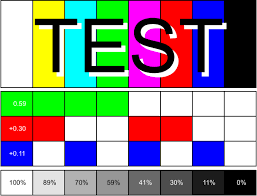
\includegraphics[width=\columnwidth]{images/test.png}
%
\section{Math Templates}
\subsection{example}
\begin{example}
    \textbf{Beispiele}
	\begin{itemize}
		\item $\Omega = \left\{\frac{1}{n}\mid n\in \mathbb{N}\right\}$\\[3pt]
		$sup(\Omega) = 1 \hspace{1cm} inf(\Omega) = 0$
		\item$[a, b]$, $[a, b)$, $(a, b]$ und $(a, b)$ mit $a<b$\\
	    a ist jeweils das Infimum und b das Supremum
	\end{itemize}
\end{example}
%
\subsection{annotation}
\begin{annotation}{Zu zeigen:}
	\item[i)] $a_n \ge$ 0
	\item[ii)] $\lim_{n\rightarrow \infty} a_n$ =0
	\item[iii)] $a_{n+1} - a_n \le$ 0 oder $\frac{a_{n+1}}{a_n} \le $ 1
\end{annotation}
%
\subsection{equation numbered}
\begin{equation}
Q=\lim_{n\rightarrow \infty} \left \vert\frac{a_{n+1}}{a_n}\right \vert \hspace{20pt} \sum_{n=0}^{\infty}a_n
	\begin{cases}
		\text{divergiert} \hspace{5pt} &Q>1\\
		\text{konvergiert absolut} &Q<1\\
		\text{keine Aussage} &Q=1
	\end{cases}
\end{equation}
%
\subsubsection{equation unnumbered}
\begin{equation*}
Q=\lim_{n\rightarrow \infty} \left \vert\frac{a_{n+1}}{a_n}\right \vert \hspace{20pt} \sum_{n=0}^{\infty}a_n
	\begin{cases}
		\text{divergiert} \hspace{5pt} &Q>1\\
		\text{konvergiert absolut} &Q<1\\
		\text{keine Aussage} &Q=1......
	\end{cases}
\end{equation*}
equation can also easily generate overfull badness
%
\vfill\null % prevents the columns content from using the full height
\columnbreak
\section{Code Template }
\subsection{tiny c++ code from source text, made to look approximately like codeexpert}
\begin{lstlisting}[
    style= codeexpert,
    basicstyle=\tiny\color{ce_white}\ttfamily\linespread{0.8},
    ]
//
#include <iostream>
int main(){
    std::cout << "Hello World" << std::endl;
    for (int i = 0; i<10; ++i){
        if(!(i%2)) std::cout << i << " is even" << '\n';
    }
}
    /* this is a comment */
    // this is also a comment
\end{lstlisting}
%
\subsection{code in normal text size}
\begin{lstlisting}[style = codeexpert]
// code
std::cout << "hello" << '\n';
\end{lstlisting}
%
\subsection{code in Huge text size} 
\begin{lstlisting}[
    style=codeexpert,
    basicstyle=\Huge\ttfamily\color{ce_white},
    ]
// code
\end{lstlisting}
%
\subsection{code from file}
\lstinputlisting[
    style = codeexpert,
    basicstyle=\tiny\color{ce_white}\ttfamily\linespread{0.8},
    ]
        {code_snippets/hello_world.cpp}
%
\subsection{code with description}
\lstinputlisting[
    style = codeexpert,
    basicstyle=\tiny\color{ce_white}\ttfamily\linespread{0.8},
    caption={Hello World program (hello\_world.cpp)}, 
    label=hello_world,
    ]
        {code_snippets/hello_world.cpp}
 %   
\subsection{code in java, without the CodeExpert style template}
\begin{lstlisting}[
    language = java,
    basicstyle=\ttfamily,
    ]
public class HelloWorld 
{
    public static void main (String[] args)
    {
        // prints Hello World!
        System.out.println("Hello World!");
    }    
}
\end{lstlisting}
%  
\end{multicols*}
%
\end{document}